\documentclass[conference, draftcls, onecolumn]{IEEEtran}
\IEEEoverridecommandlockouts
\usepackage{tabularx}
\usepackage{algorithmic}
\usepackage{booktabs}
\usepackage{textcomp}
\usepackage{graphicx}
\usepackage{mathtools}
\graphicspath{ {./imgs/} }

\usepackage{amssymb,latexsym,amsmath}
\allowdisplaybreaks
\usepackage[style=ieee]{biblatex}
\addbibresource{LiamBibliography.bib}

\usepackage{amsthm}
\usepackage{enumitem}
\usepackage{float}
\usepackage[hidelinks]{hyperref}
\usepackage{multirow}
\algsetup{linenodelimiter=\ }
\renewcommand{\algorithmiccomment}[1]{(#1)}

\newtheorem{theorem}{Theorem}
\newtheorem{corollary}{Corollary}
\newtheorem{proposition}{Proposition}
\newtheorem{lemma}{Lemma}
\newtheorem{definition}{Definition}
\newtheorem{assumption}{Assumption}

\allowdisplaybreaks

\DeclareMathOperator*{\argmax}{argmax}
\DeclareMathOperator*{\argmin}{argmin}

\def\BibTeX{{\rm B\kern-.05em{\sc i\kern-.025em b}\kern-.08em
    T\kern-.1667em\lower.7ex\hbox{E}\kern-.125emX}}

\begin{document}
\title{Reinforcement Learning for Zero-Delay Coding of Markov Sources
    \thanks{Research is supported by the Natural Sciences and Engineering Research Council of Canada. The first author was supported by a Queen's University Department of Mathematics and Statistics Summer Research Award.}
}

\author{\IEEEauthorblockN{Liam Cregg}
    \IEEEauthorblockA{\textit{Mathematics and Statistics} \\
        \textit{Queen's University}\\
        Kingston, Canada \\
        liam.cregg@queensu.ca}
    \and
    \IEEEauthorblockN{Tam\'as Linder}
    \IEEEauthorblockA{\textit{Mathematics and Statistics} \\
        \textit{Queen's University}\\
        Kingston, Canada \\
        tamas.linder@queensu.ca}
    \and
    \IEEEauthorblockN{Serdar Y\"uksel}
    \IEEEauthorblockA{\textit{Mathematics and Statistics} \\
        \textit{Queen's University}\\
        Kingston, Canada \\
        yuksel@queensu.ca}}

\maketitle

\begin{abstract}
    In the classical lossy coding problem, one is allowed to encode long sequences of source symbols in order to achieve a lower distortion. This is undesirable in many delay-sensitive applications. Accordingly, we consider the zero-delay case where one wishes to encode a source symbol causally. It has been shown that this problem lends itself to stochastic control techniques, leading to existence and structural results. However, attempting to develop analytical solutions or algorithmic implementation using these methods has been computationally difficult. To that end, we propose a reinforcement learning approach. First, we will establish some supporting results on regularity and stability properties. Afterwards, building on recent results on quantized Q-learning, we show that a quantized Q-learning algorithm can be used to obtain a near-optimal policy for this problem. Finally, we provide some relevant simulation results.
\end{abstract}

% Intro to zero-delay coding / motivation
% Past work, in particular reference Witsenhausen, Walrand & Varaiya, Tamas, Serdar, Richard
% Main contribution
% Intro to zero-delay quantizers, summarize results from "Zero-Delay Lossy Coding"
\section{Introduction}\label{section:introduction}
\subsection{Zero-Delay Lossy Coding}
We consider the problem of encoding an information source without delay, sending the encoded source over a discrete noiseless channel, and recontructing the source at the decoder (also without delay). That is, the classical block-coding approach is not viable. We will also allow the encoder to have access to feedback from the channel. Formally, the setup is as follows:

The source \( \{X_t\}_{t \ge 0} \) is a time-homogeneous, discrete-time Markov process taking values in a finite set \(\mathbb{X}\). Assume that the source is irreducible and aperiodic (and thus admits a unique invariant measure), and has transition kernel \( P(x_{t+1} | x_t) \). We also assume that the distribution of \(X_0\), which we denote by \(\pi_0\), is available at the encoder and decoder. After encoding, the (compressed) information, denoted by \(q_t\), is sent over a discrete noiseless channel with input and output alphabets \( \mathcal{M} := \{1,\ldots,M\} \). Thus, the encoder is defined by an encoder policy \( \gamma^e = \{\gamma^e_t\}_{t \ge 0} \), where \( \gamma^e_t : \mathcal{M}^t \times \mathbb{X}^{t+1} \to \mathcal{M} \), and \(q_t = \gamma^e_t(q_{[0,t-1]},X_{[0,t]})\), where we use the notation \(X_{[0,t-1]} = (X_0, \ldots, X_{t-1})\), etc. Then, the decoder generates the reconstruction \( \hat{X}_t \) without delay, using decoder policy \( \gamma^d = \{\gamma^d_t\}_{t \ge 0} \), where \( \gamma^d_t : \mathcal{M}^{t+1} \to \hat{\mathbb{X}} \). Thus we have \( \hat{X}_t = \gamma^d_t(q_{[0,t]}) \).

Note that for fixed \(q_{[0,t-1]}\) and \(X_{[0,t-1]}\), the map \(\gamma^e_t(q_{[0,t]}, X_{[0,t-1]}, \cdot)\) is a \emph{quantizer} (i.e. a map from \(\mathbb{X}\) to \(\mathcal{M}\), which we denote by \(Q_t\). So we can view an encoder policy at time \(t\) as selecting a quantizer \(Q_t\), then quantizing \(q_t = Q_t(X_t)\).

Also, since the source alphabet is finite, there exists an optimal decoding policy for every encoding policy. Thus we will denote the encoding policy by \( \gamma := \gamma^e \), and assume it is paired with an optimal decoding policy. We can then restrict our search only to optimal encoding policies.

In general, for the zero-delay coding problem, the goal is to minimize the average-cost/distortion. In the infinite-horizon case, this is given by: %chktex 9
\[ J(\pi_0, \gamma) := \limsup_{T\to\infty}\mathbf{E}_{\pi_0}^{\gamma}\left[\frac{1}{T}\sum_{t=0}^{T-1}d(X_t,\hat{X}_t)\right]\label{eq:average_cost}, \]

where \(d : \mathbb{X} \times \hat{\mathbb{X}} \to \mathbb{R}\) is some distortion function and \(\mathbf{E}_{\pi_0}^{\gamma}\) is the expectation with \(X_0 \sim \pi_0\) and under encoder policy \(\gamma\). We denote the optimal average cost by \(J^*(\pi_0) := \inf_{\gamma \in \Gamma}J(\pi_0,\gamma)\), where \(\Gamma\) is the set of all admissible encoder policies.

\subsection{Literature Review}
A number of important structural results have been obtained under this setup. In particular, for the finite horizon problem, \cite{Witsenhausen} showed that any encoder policy can be replaced, without performance loss, by one using only \(q_{[0,t-1]}\) and \(X_t\) to generate \(q_t\). Furthermore, \cite{Walrand} proved a similar result for an encoder policy using only the conditional probability \(P(X_t \in \cdot | q_{[0,t-1]})\) and \(X_t\). These results were generalized in further papers, see e.g.~\cite{Teneketzis, MahTen09, YukIT2010arXiv, Linder, Wood}. Of particular interest for us are the results from~\cite{Wood}, which considered existence of optimal policies in the infinite-horizon case. Formally, we introduce the following:

Let \(\mathcal{P}(\mathbb{X})\) be the space of probability measures on \(\mathbb{X}\), and define \(\pi_t \in \mathcal{P}(\mathbb{X})\) as:
\[\pi_t(A) := \text{Pr}(X_t \in A | q_{[0,t-1]})\]

\begin{definition}
    We say an encoder policy \(\gamma = \{\gamma_t\}_{t\ge0}\) is of the \textbf{Walrand-Varaiya type} if, at time \(t\), the policy uses only \(\pi_t\) and \(X_t\) to generate \(q_t\). That is, \(\gamma\) selects a quantizer \(Q_t = \gamma_t(\pi_t)\) and \(q_t\) is generated as \(q_t = Q_t(X_t)\).
\end{definition}

Such a policy is called \emph{stationary} if it does not depend on \(t\), i.e. \(\gamma_t\) is a fixed policy.

\begin{theorem}\label{theorem:Wood}\cite[Theorem 3]{Wood}
    There exists a stationary Walrand-Varaiya type policy \(\gamma^*\) that solves the infinite-horizon average-cost problem, i.e. one that satisfies:
    \[J(\pi_0,\gamma^*) = J^*(\pi_0)\]
    for all \(\pi_0\).
\end{theorem}

We note that, despite the key structural results obtained for this problem, finding an optimal policy (either algorithmically or analytically) is difficult. Under certain assumptions on the source and channel, solutions have been found. For example, \cite{Walrand} showed memoryless encoding is optimal when \(\mathbb{X} = \mathcal{M}\) and the channel is symmetric, and \cite{Tatikonda2004} studied the Gauss-Markov source when the channel satisfies certain ``matching'' properties. However, for a general source and channel, finding an optimal encoding policy is an open problem.

We also note the importance of stochastic control approaches in the above structural results. Indeed, under a stochastic control framework, \cite{Witsenhausen, Walrand} use a dynamic programming recursion in their study of the finite horizon problem, a convex analytic method is employed in~\cite{Linder}, and \cite{Wood, Tatikonda2009} study the average-cost optimality equation. In keeping with this strategy, we propose to use a reinforcement learning approach often used to find solutions to stochastic control problems. In particular, we will use results from~\cite{Kara} to rigorously justify convergence of this algorithm to a near-optimal solution.

In our study of the average-cost problem, we will make use of the discounted-cost problem. That is, for some \( \beta \in (0,1) \), we wish to minimize:
\[ J_{\beta}(\pi_0, \gamma) := \lim_{T\to\infty}\mathbf{E}_{\pi_0}^{\gamma}\left[\sum_{t=0}^{T-1}\beta^t d(X_t,\hat{X}_t)\right]\label{eq:discounted_cost} \]

And as with the average cost, we denote the optimal discounted cost by \(J_\beta^*(\pi_0) := \inf_{\gamma \in \Gamma}J_\beta(\pi_0,\gamma)\). Note that the discounted-cost problem is in general not very interesting from a source coding perspective. However, we will need it for the rigorous proof of convergence, and we will relate the discounted-cost problem to the average-cost one. For this reason, we also introduce the following result from~\cite{Wood}.

\begin{theorem}\label{theorem:Wood2}\cite[Proposition 2]{Wood}
    There exists a stationary Walrand-Varaiya type policy \(\gamma^*\) that solves the infinite-horizon discounted-cost problem, i.e. one that satisfies:
    \[J_\beta(\pi_0,\gamma^*) = J_\beta^*(\pi_0)\]
    for all \(\pi_0\).
\end{theorem}

Under certain assumptions, as \(\beta \to 1\), the optimal discounted-cost (with an appropriate normalization) approaches the optimal average-cost. We will use Theorem~\ref{theorem:ACOE} in the Appendix. The assumptions of this theorem have been shown to hold; in particular, \cite[Lemma 11]{Linder} and \cite[Lemma 1]{Wood} give parts (3) and (5), while the rest will follow from our setup of the problem in Section~\ref{section:optimal quantizers}. By Theorem~\ref{theorem:ACOE}, we have that there exists some sequence \(\{\beta_n\}_{n \ge 0}\) with \(\beta_n \to 1\) such that:
\[J^*(\pi_0) = \lim_{n \to \infty}(1-\beta_n)J^*_{\beta_n}(\pi_0)\]

Therefore, we may approximate the optimal average cost using the discounted cost. Hence, we will develop an algorithm for the discounted-cost problem which yields a near-optimal policy, and if we do this for large enough \(\beta\), we obtain a cost close to the optimal average cost.

The remainder of the paper is organized as follows:
\begin{itemize}
    \item In Section~\ref{section:optimal quantizers} we formulate the zero delay coding problem as a Markov decision process (MDP) and review key results from~\cite{Linder, Wood}.
    \item Section~\ref{section:Q-learning} introduces our proposed Q-learning solution, based on results from~\cite{Kara}.
    \item In Section~\ref{section:unique-ergodicity}, we prove additional regularity properties of our MDP and relate them to the above Q-learning solution.
    \item Section~\ref{section:Algorithms} contains the final algorithm and a rigorous justification of convergence to a near-optimal policy for the discounted-cost problem (which is related to the average-cost problem through Theorem~\ref{theorem:ACOE}).
    \item Finally, Section~\ref{section:results} provides some simulation results and a comparison to other encoder policies.
\end{itemize}

\section{Optimal Quantizers}\label{section:optimal quantizers}

Under Walrand-Varaiya type policies, it was shown in~\cite{Linder} that \( \{\pi_t\} \) is a controlled Markov process with control \( \{Q_t\} \). More specifically, we have the following result:
\begin{proposition}\cite{Linder}
    Under a Walrand-Varaiya type policy, the update equation for \(\pi_t\) is given by
    \begin{equation}
        \pi_{t+1}(x_{t+1}) = \frac{1}{\pi_t(Q_t^{-1}(q_t))}\smashoperator[r]{\sum_{x_t \in Q_t^{-1}(q_t)}}P(x_{t+1}|x_t)\pi_t(x_t)\label{eq:1}
    \end{equation}
    Therefore \( \pi_{t+1} \) is conditionally independent of \( (\pi_{[0,t-1]}, Q_{[0,t-1]}) \) given \( \pi_t \) and \( Q_t \), and hence \( \{\pi_t\} \) is a controlled Markov process with control \( \{Q_t\} \).
\end{proposition}

We will denote the transition kernel induced by the above update equation by \( P(d\pi_{t+1} | \pi_t, Q_t) \) (this is a distribution on \( \mathcal{P(\mathbb{X})}) \). We also define the following cost function for this process in terms of \( \pi_t \) and \( Q_t \) (this is the average distortion if the optimal decoder is used for a given \(Q_t\)).

\begin{equation}\label{eq:cost}
    c(\pi_t, Q_t) := \sum_{i=1}^M \min_{\hat{x} \in \hat{\mathbb{X}}} \sum_{x \in Q_t^{-1}(i)} \pi_t(x)d(x,\hat{x})
\end{equation}

Note that by this definition of \( c(\pi_t,Q_t) \) and our assumption that we are using an optimal decoder for a given encoder of the optimal Walrand-Varaiya type, we have:
\[\mathbf{E}_{\pi_0}^{\gamma}\left[\frac{1}{T}\sum_{t=0}^{T-1}c(\pi_t,Q_t)\right] = \mathbf{E}_{\pi_0}^{\gamma}\left[\frac{1}{T}\sum_{t=0}^{T-1}d(X_t,\hat{X}_t)\right]\]

% Motivation: value iterations etc. is very difficult (not just computationally but also algorithm design, given the setup of problem)
%In theory one could use dynamic programming principles to run an iterative algorithm on this controlled Markov process in order to obtain the optimal policy. However, in practice this proves to be difficult (see e.g.~\cite{Wood}), and hence we propose to use Q-learning in order to find the optimal quantization policy. To this end, we will utilize the recent work of~\cite{Kara} in the near-optimality of policies obtained through Q-learning under quantization.

\subsection{A Topology on Quantizers}
As we will be discussing convergence and continuity regarding quantizers, we need to define an appropriate topology. Let \( Q : \mathbb{X} \to \mathcal{M}\) be a quantizer, and denote the \( i^{th} \) \emph{bin} of \( Q \) by \( B_i = Q^{-1}(i), i \in \mathcal{M} \). We denote the set of all possible quantizers by \( \mathcal{Q} \) (since \(\mathbb{X}\) and \(\mathcal{M}\) are finite, so is \(\mathcal{Q}\)). Following~\cite{YukselOptimizationofChannels,Linder}, we note that \(Q\) can alternatively be represented as a stochastic kernel from \( \mathbb{X} \) to \( \mathcal{M} \) such that \( Q(i|x) = 1_{\{x \in B_i\}}, i \in \mathcal{M} \). Then for \( P \in \mathcal{P}(\mathbb{X}) \), we denote by \( PQ \) the joint probability measure \( PQ(x,y) = P(x)Q(y|x), (x,y) \in \mathbb{X} \times \mathcal{M} \). If we introduce the equivalence relation \( Q \equiv Q' \) iff \( PQ = PQ' \), then we can imbue the equivalence classes with the weak convergence topology (that is, we say \( Q_n \to Q \) weakly iff \( PQ_n \to PQ \) weakly). Under this topology,~\cite{Linder} showed the following property of the controlled Markov chain \( \{\pi_t\} \).

\begin{lemma}\label{lemma:weak}~\cite[Lemma 11]{Linder}.
    The transition kernel \( P(d\pi_{t+1}|\pi_t,Q_t) \) is weakly continuous in \( (\pi_t,Q_t) \). That is,

    \[ \int_{\mathcal{P}(\mathbb{X}) \times \mathcal{Q}} f(\pi^{'})P(d \pi^{'}|\pi, Q) \]

    is continuous on \( \mathcal{P}(\mathbb{X}) \times \mathcal{Q} \) for all continuous bounded \(f\).
\end{lemma}

\noindent We briefly remark on the setup so far.
\vspace{1em}

\noindent\emph{Remark 1.}\label{remark:1}
\begin{enumerate}[wide, labelwidth=!, labelindent=0pt]
    \item We now have a controlled Markov chain \(\{\pi_t\}\), which takes values in \(\mathcal{P}(\mathbb{X})\), with \(\mathcal{Q}\)-valued control \(\{Q_t\}\). Equipped with the cost function~\eqref{eq:cost}, this becomes a Markov decision process (MDP) (see Section~\ref{section:Q-learning} and \cite{Lerma} for more information on MDPs). Theorem~\ref{theorem:Wood} tells us that solving the zero delay coding problem is equivalent to finding an optimal policy Walrand-Varaiya type policy for this MDP.
    \item We wish to use a reinforcement learning approach to find an optimal or near-optimal policy for this MDP. We note that, although our information source \(\mathbb{X}\) is finite, the state space for our new MDP is \(\mathcal{P}(\mathbb{X})\) and therefore uncountable. We will see how this impacts reinforcement learning in the following section.
\end{enumerate}


% Intro to quantized Q-learning, summarize results from "Q-learning for General Spaces"
\section{Q-learning and Quantized Q-learning}\label{section:Q-learning}

\subsection{Q-learning for Finite Models}
As in~\cite[Chapter 2]{Lerma}, we define a \emph{Markov decision process} as a 4-tuple \((\mathsf{X},\mathsf{U},P,c)\), where:
\begin{enumerate}
    \item \(\mathsf{X}\) is the \emph{state space}, which we assume is Polish (i.e. a Borel subset of a complete, separable metric space).
    \item \(\mathsf{U}\) is the \emph{action space}, also Polish.
    \item \(P = P(\cdot|x,u)\) is the \emph{transition kernel}, a stochastic kernel on \(\mathsf{X}\) given \(\mathsf{X} \times \mathsf{U}\).
    \item \(c : \mathsf{X} \times \mathsf{U} \to [0,\infty)\) is the \emph{cost function}.
\end{enumerate}

For now, we will assume \(\mathsf{X}\) and \(\mathsf{U}\) are both finite, and deal with the infinite case shortly. An \emph{admissible policy} is a sequence \(\gamma = \{\gamma_t\}_{t\ge0}\) such that \(\gamma_t : \mathsf{U}^t \times \mathsf{X}^{t+1} \to \mathsf{U}\). Such a policy, along with the transition kernel \(P\) and an initial distribution \(X_0 \sim \mu\), define a unique distribution for \((X_t,U_t)_{t\ge0}\). The goal (for the infinite-horizon, discounted-cost case) is to find a policy \(\gamma\) minimizing:
\[J_\beta(\mu,\gamma) := \lim_{T\to\infty}E^\gamma_\mu\left[\sum_{t=0}^{T-1}\beta^t c(X_t,U_t) \right]\]
for some \(\beta \in (0,1)\).

We define the optimal value function as the above cost when an optimal policy is used:
\[J_\beta^*(\mu) := \inf_{\gamma}J_\beta(\mu,\gamma)\]

We also note that if \(\mu = \delta_x\), we denote the above by \(J_\beta^*(x)\). A key result in stochastic control theory is that a function is the optimal value function iff it satisfies the discounted-cost optimality equation (DCOE):
\begin{equation} J_\beta^*(x) = \min_{u\in\mathsf{U}}\biggl\{ c(x,u) + \beta\sum_{y \in \mathsf{X}}J^*_\beta(y)P(y | x,u) \biggl\}\label{eq:DCOE} \end{equation}

A common method to find a policy satisfying the DCOE is Q-learning, which we now define. Here, \(\mathsf{Q}_t : \mathsf{X} \times \mathsf{U} \to \mathbb{R} \) is the \emph{Q-factor} at time \(t\ge0\), and \(\alpha_t : \mathsf{X} \times \mathsf{U} \to \mathbb{R}\) is the \emph{learning rate}. Suppose that we start at an arbitrary \(\mathsf{Q}_0\) and we use some arbitrary admissable policy \(\gamma\). The Q-factors are updated as follows:

\vspace{1em}

\noindent \underline{\textbf{Q-learning}}\label{algorithm:Q-learning}

\begin{algorithmic}[1]
    \STATE Initialize \(x_0\) according to \(\mu\)
    \FOR{\(t\ge0\)}
    \STATE \(u_t = \gamma_t(x_t)\)
    \IF{\((x,u) = (x_t,u_t)\)}
    \STATE \(\mathsf{Q}_{t+1}(x,u) = (1- \alpha_t(x,u))\mathsf{Q}_t(x,u) + \alpha_t(x,u)[c(x,u)+\beta \; \underset{v\in\mathbb{U}}{\text{min}} \; \mathsf{Q}_t(X_{t+1},v)]\)
    \ELSE
    \STATE \(\mathsf{Q}_{t+1}(x,u) = \mathsf{Q}_t(x,u)\)
    \ENDIF
    \STATE Receive \(x_{t+1}\) according to \(P(\cdot | x_t, u_t)\)
    \ENDFOR
\end{algorithmic}

We impose the following assumption on the learning rate \(\alpha_t\).

\begin{assumption}\label{assumption:alpha}
    For all \((x,u) \in \mathsf{X} \times \mathsf{U}\) and for all \(t\ge0\), we have
    \begin{enumerate}
        \item \(\alpha_t(x,u) \in [0,1]\).
        \item \(\alpha_t(x,u) \) is a function of \((x_0,u_0),\ldots,(x_t,u_t)\).
        \item \(\sum_{t\ge0}\alpha_t(x,u) = \infty\).
        \item \(\sum_{t\ge0}\alpha_t^2(x,u) < \infty\).
    \end{enumerate}
\end{assumption}

A well-known result in stochastic control theory is the following:
\begin{proposition}\cite{Watkins}
    Under Assumption~\ref{assumption:alpha}, in the above algorithm the Q-factors \(\{\mathsf{Q}_t\}_{t\ge0}\) converge almost surely to:
    \[\mathsf{Q}^*(x,u) := c(x,u) \\ + \beta\sum_{y \in \mathsf{X}}\min_{v\in\mathsf{U}}\bigl\{\mathsf{Q}(y,v)\bigl\}P(dy | x,u)\]
\end{proposition}

Note that \(\min_{v \in \mathsf{U}}\mathsf{Q}^*(x,v) = J^*_\beta(x)\) and hence the policy made up of these minimizing actions is optimal. Although a powerful algorithm, we cannot apply this to our zero-delay coding problem directly as our state space is infinite, and therefore (3) in Assumption~\ref{assumption:alpha} will fail. A potential solution is to use ``quantized'' Q-learning - that is, we approximate the original MDP using some other MDP with a finite state space, and run Q-learning on this model. Under some additional assumptions, \cite{Kara} showed that one can indeed achieve near-optimality for the original MDP in this fashion. Note that \cite{Kara} also considered quantization of the action space, but we will not need this for our application, and so we will assume \(\mathsf{U}\) is finite.

\subsection{Finite Model Approximations: State Space}
\begin{assumption}\label{assumption:MDP} Our original MDP has the following properties:
    \begin{enumerate}
        \item The stochastic kernel \(P(\cdot | x,u)\) is weakly continuous in (x,u), i.e. \(P(\cdot | x_n,u_n) \to P(\cdot | x,u)\) weakly for all \((x_n,u_n) \to (x,u)\).
        \item The cost function \(c\) is continuous and bounded.
        \item The action space \(\mathsf{U}\) is finite.
        \item The state space \(\mathsf{X}\) is \(\sigma\)-compact.
    \end{enumerate}
\end{assumption}

Let \(\{B_i\}_{i=1}^N\) be a partition of \(\mathsf{X}\), and let \(\mathsf{Y} := \{y_1,\ldots,y_N\}\) where \(y_i \in B_i\). We define a \emph{quantizer} on \(\mathsf{X}\) as a mapping \(f : \mathsf{X} \to \mathsf{Y}\), such that
\[ f(x) = y_i \quad \text{if} \; x \in B_i \]

Now let \(\psi \in \mathcal{P}(\mathsf{X})\). Then with an abuse of notation we define the resulting conditional distribution
\[\psi(A | y_i) := \frac{\psi(A)}{\psi(B_i)}\]

Let \(\hat{\text{MDP}} := (\mathsf{Y}, \mathsf{U}, \hat{c}, \hat{P})\), where \(\hat{c}\) and \(\hat{P}\) are defined as the mean of the original \(c\) and \(P\) over the quantization bins. That is:
\begin{gather} \nonumber \hat{c}(y_i,u) := \int_{B_i}c(x,u)\psi(dx | y_i) \\
    \hat{P}(y_j | y_i,u) := \int_{B_i}P(B_j | x,u)\psi(dx | y_i)\label{eq:hats}\end{gather}

Then let \(\hat{J}_\beta\) be the optimal value function for \(\hat{\text{MDP}}\), and note that we can extend this function over \(\mathsf{X}\) by making it constant over each \(B_i\), i.e.
\[ \hat{J}_\beta(x) := \hat{J}_\beta(y_i) \quad \forall x \in B_i \]

We also define:
\[ d_\infty := \max_{i=1,\ldots,N-1} \sup_{x,x' \in B_i}||x-x'||\].

And note that under Assumption~\ref{assumption:MDP}, \(\mathsf{X}\) is \(\sigma\)-compact, and hence there exists a sequence of partitions \(\{B_i\}_{i=1}^N\) such that \(d_\infty \to 0\) and \(\bigcup_{i=1}^{N-1}B_i \uparrow \mathsf{X}\) as \(N \to \infty\). Then we have:

\begin{theorem}\label{theorem:2.3}\cite[Theorem 4.27]{Quantized_Models}
    Under Assumption~\ref{assumption:MDP}, we have for all compact \(K \subset \mathsf{X}\) and as \(d_\infty \to 0\),
    \[ \sup_{x_0 \in K}|\hat{J}_\beta(x_0) - J^*_\beta(x_0)| \to 0 \]
    and
    \[ \sup_{x_0 \in K}|J_\beta(x_0,\hat{\gamma}) - J^*_\beta(x_0)| \to 0 \]
    where \(\hat{\gamma}\) is the optimal policy of \(\hat{\text{MDP}}\) extended to \(\mathsf{X}\).
\end{theorem}

\subsection{Quantized Q-learning}
Based on the above theorems, we can find a near-optimal policy for the discounted-cost problem by quantizing our state space finely enough, and finding an optimal policy for \(\hat{\text{MDP}}\). However, we do not necessarily know that a Q-learning algorithm for this new MDP will converge, as the quantization process introduces some non-Markovian features into the MDP~\cite{Kara}. A result from~\cite{Kara} does in fact guarantee convergence of a Q-learning algorithm to the optimal Q-factor of \(\hat{\text{MDP}}\) under some additional assumptions. The algorithm is exactly as the \hyperref[algorithm:Q-learning]{\textbf{Q-learning}} algorithm, but with \(\mathsf{Q}_t : \mathsf{Y} \times \mathsf{U}\) and \(\alpha_t : \mathsf{Y} \times \mathsf{U} \to \mathbb{R}\). That is, line 5 becomes:
\begin{equation}\mathsf{Q}_{t+1}(f(x),u) = (1- \alpha_t(f(x),u))\mathsf{Q}_t(f(x),u) +
    \alpha_t(f(x),u)(c(x,u)+\beta \; \underset{v\in\mathsf{U}}{\text{min}} \; \mathsf{Q}_t(f(X_{t+1}),v))\label{eq:Q-factor-quantized}\end{equation}

\begin{assumption}\label{assumption:Q-learning} In the above Q-learning algorithm, we have:
    \begin{enumerate}
        \item \[\alpha_t(y,u) = \begin{cases}
                      \frac{1}{1 + \sum_{k=0}^t 1_{(Y_k,U_k) = (y,u)}} & (Y_t,U_t) = (y,u) \\
                      0                                                & otherwise
                  \end{cases}\]
        \item The policy \(\gamma\) chooses control actions independently of everything and randomly, i.e.
              \[ \textup{Pr}(\gamma(\cdot) = u_i) = p_i \quad \forall i = 1,\ldots,|\mathsf{U}| \]
              where \(p_i > 0 \; \forall i\) and \(\sum_i p_i = 1\).
        \item Under the above policy \(\gamma\), the state process \(\{X_t\}_{t\ge0}\) admits a unique invariant measure \(\psi^*\).
    \end{enumerate}
\end{assumption}

\begin{theorem}\label{theorem:convergence}\cite[Theorem 3.2]{Kara}
    Under Assumption~\ref{assumption:Q-learning}, for each \((y_i,u) \in \mathsf{Y} \times \mathsf{U}\), \(Q_{t+1}(y_i, u)\) in~\eqref{eq:Q-factor-quantized} converges to:
    \[ Q^*(y_i,u) = \hat{c}(y_i,u) + \beta \sum_{y_j \in \mathbb{Y}}\hat{P}(y_j | y_i,u)\min_{v \in \mathbb{U}}Q^*(y_j,v), \]
    where \(\hat{c}\) and \(\hat{P}\) are defined as in~\eqref{eq:hats} with \(\psi = \psi^*\).
\end{theorem}

We remark briefly on the connection of this quantized Q-learning to our original zero-delay coding problem:

\vspace{1em}
\noindent\emph{Remark 2.}\label{remark:2}
\begin{enumerate}[wide, labelwidth=!, labelindent=0pt]
    \item We were able to reduce the zero-delay coding problem to an MDP in Section~\ref{section:optimal quantizers}, but the MDP had an infinite state space, and thus it was impossible to use standard Q-learning on it (recall that this MDP had \(\pi_t\), a probability distribution, as its state).
    \item Given the above theorems, we can use a quantized Q-learning algorithm to find a near-optimal policy for this MDP. We just need to confirm that Assumption~\ref{assumption:MDP} and Assumption~\ref{assumption:Q-learning} hold. Indeed, from Lemma~\ref{lemma:weak} and the definition of \(c\), we already have that Assumption~\ref{assumption:MDP} holds. Parts (1) and (2) of Assumption~\ref{assumption:Q-learning} are determined by algorithm design, and so can be met. We are thus left with proving that part (3) is met, i.e. that the process \(\{\pi_t\}_{t\ge0}\) admits a unique invariant measure under a random exploration policy. The next section is dedicated to showing this fact.
\end{enumerate}

\section{Unique Ergodicity Under a Memoryless Exploration Policy}\label{section:unique-ergodicity}
Recall our setup from Section~\ref{section:optimal quantizers}. In particular, we have a controlled Markov process \(\{\pi_t\}_{t\ge0}\), with control \(\{Q_t\}_{t\ge0}\), where \(Q_t : \mathbb{X} \to \mathcal{M}\). Here \(\mathbb{X}\) is our source alphabet, \(\mathcal{M}\) is our message set, and we have \(Q_t(X_t) = q_t\) as the quantizer output.

We wish to show that if we choose the \(Q_t\) randomly, \( \{\pi_t\}_{t\ge0} \) admits a unique invariant measure. Note that under a random exploration policy, we can view a given quantizer output \(q_t \in \mathcal{M}\) as an observation of the true state \( X_t \), dependent on an i.i.d. noise variable \( Z_t\). That is, we enumerate the set of quantizers as \(\mathcal{Q} = \{Q_1,\ldots,Q_m\} \). Then let \( q_t = h(x_t,z_t) = Q_{z_t}(x_t) \), where \( Z_t \) is an i.i.d random variable taking values in \( \mathcal{Z} := \{1,\ldots,m\} \), with \(Z_0 \sim R\) positive everywhere. Then we can use some tools from the literature of Partially Observed Markov Processes (POMPs) to study the ergodicity of \( \{\pi_t\} \).

\subsection{Predictor and Filter Merging}

%For a fixed \( x \in \mathbb{X} \), we denote \( h(x,\cdot) := h_x(\cdot) : \mathcal{Z} \to \mathbb{Y} \), and let \( \{Z_t\}_{t\ge0} \) have probability measure \( Z_0 \sim R \) where \(R\) is positive everywhere. The noise process is independent of the state process \( \{X_t\}_{t\ge0} \), so we can write the following update equation for the joint process \( \{X_t,Y_t\}_{t\ge0} \)

%\[ P((X_{t+1},Y_{t+1}) | (X,Y)_{[0,t]} = (x,y)_{[0,t]}) = R(h_{x+1}^{-1}(y_{t+1}))P(x_{t+1} | x_t) \]

%It follows that \( \{X_t,Y_t\}_{t\ge0} \) is Markov, with a probability measure on \( \mathbb{X}^{\mathbb{Z}_{\ge0}} \times \mathbb{Y}^{\mathbb{Z}_{\ge0}} \), endowed with the product topology. Since this measure depends on the distribution of \( X_0 \), we denote this measure by \( P^\mu \) where \( X_0 \sim \mu \).

Given the above characterization, we can view \( \pi_t \) as what is known as a \emph{predictor} in the POMDP literature. Recall the recursion equation~\eqref{eq:1} and note that this is dependent on the initialization of \( \pi_0 \), also called the \emph{prior}. We denote the predictor process resulting from the prior \( \pi_0 = \nu \) as \( \{\pi_t^\nu \}_{t\ge0} \). A common question in the POMDP literature is when measures such as the predictor are \emph{stable}. More formally, we introduce the following definitions:

\begin{definition}\label{definition:weak_stable}
    A predictor process \(\{\pi_t\}_{t\ge0}\) is stable in the sense of weak merging in expectation if for any \( f \in C_b(\mathbb{X}) \) and any prior \( \nu \) with \( \mu \ll \nu \), we have \( \lim_{n \to \infty}E^\mu [|\int fd\pi_t^\mu - \int fd\pi_t^\nu|] = 0 \).
\end{definition}

\begin{definition}\label{definition:TV_stable}
    A predictor process \(\{\pi_t\}_{t\ge0}\) is stable in the sense of total variation in expectation if for any prior \( \nu \) with \( \mu \ll \nu \), we have \( \lim_{n \to \infty}E^\mu [||\pi_t^\mu - \pi_t^\nu||_{TV}] = 0 \). Here \( ||A-B||_{TV} = \sup_{||f||_\infty \le 1} |\int fdA - \int fdB| \) for f measurable.
\end{definition}

Note that Definition~\ref{definition:TV_stable} is stronger than Definition~\ref{definition:weak_stable}. The following result follows from~\cite[Theorem 2]{Stettner}, and making use of the above structure of \(q_t\). The proof can be found in the Appendix.

\begin{theorem}\label{theorem:unique}
    Suppose the following hold:
    \begin{enumerate}
        \item There exists a unique invariant measure \( \zeta(dx) \) for the Markov process \( \{X_t\}_{t\ge0} \).
        \item The predictor process \( \{\pi_t\}_{t\ge0} \) is stable in the sense of Definition~\ref{definition:weak_stable}.
        \item The joint process \( \{X_t,\pi_t \}_{t\ge0} \) is Feller.
    \end{enumerate}
    Then the process \(\{\pi_t\}_{t\ge0}\) admits a unique invariant measure.
\end{theorem}

Note that in our setup in Section~\ref{section:introduction}, we assumed \( \{X_t\}_{t\ge0} \) admits a unique invariant measure, so (1) is met. Furthermore, since \(\mathbb{X}\) is finite and \(\{\pi_t\}_{t\ge0}\) is Feller by Lemma~\ref{lemma:weak} (see \cite[Definition C.3]{Lerma}), we have that \(\{X_t,\pi_t \}_{t\ge0}\) is Feller, so (3) is met. Then we are left with showing (2).

\subsection{Predictor Stability}
To show predictor stability, we will utilize results in~\cite{Curtis}, which relate the stability of the predictor to stability of the \emph{filter}, which we denote by \(\pi^*_t\). The filter has the same form as the predictor but is further conditioned on \( q_t \) (that is, \( \pi_t^* = P(x_t | q_{[0,t]}) \)). We have the following result.

\begin{lemma}\label{lemma:filter-predictor}\cite[Theorem 2.11]{Curtis}
    The filter merges in total variation in expectation if and only if the predictor merges in total variation in expectation.
\end{lemma}

And finally, we show that the filter is stable in total variation in expectation. Recall that we defined \(q_t = h(x_t,z_t) = Q_{z_t}(x_t)\), where \(Q_{z_t}\) was our random quantizer choice. Then we denote \(h_x(\cdot) := h(x,\cdot)\). The following lemma is originally from~\cite{Handel}, which was presented in a more general context.

\begin{lemma}\label{lemma:nondegenerate}\cite[Corollary 5.5]{Handel}
    Consider the conditional probability measure defined by \( R(h_x^{-1}(q)) \). If this is strictly positive for all \((x,q)\), then the filter converges in total variation in expectation.
\end{lemma}

To show that this density is positive in the quantizer case, recall that under a memoryless exploration policy we have that \(R\) is positive everywhere. Then, since \( \mathcal{Q} \) contains every posssible quantizer \( Q : \mathbb{X} \to \mathcal{M} \), we have that for all \( (x,q) \), there exists at least one quantizer such that \( Q(x) = q \), and thus \( h_x^{-1}(q) \) is nonempty for all \( (x,q) \). Then, since \(R\) is positive everywhere, we obtain by Lemma~\ref{lemma:nondegenerate} that the filter is stable in total variation in expectation.

Note that the above arguments also hold as long as, for all \( (x,q) \), our set of quantizers contains \emph{at least one} quantizer \( Q \) st \( Q(x) = q \). More concretely, we impose the following assumption on our set of quantizers \( \mathcal{Q} \).

\begin{assumption}\label{assumption:one-bin}
    For all \((x,q)\), we have \(\{Q \in \mathcal{Q} : Q(x) = q\} \neq \emptyset\).

\end{assumption}

\noindent To summarize, we have the following theorem.

\begin{theorem}\label{theorem:invariant}
    If the set of quantizers \( \mathcal{Q} \) satisfies Assumption~\ref{assumption:one-bin}, then under any memoryless exploration policy, the Markov process \( \{\pi_t\}_{t\ge0} \) admits a unique invariant measure.
\end{theorem}

\begin{proof}
    First, under Assumption~\ref{assumption:one-bin} and by Lemma~\ref{lemma:nondegenerate}, the filter is stable in total variation in expectation. Then, by Lemma~\ref{lemma:filter-predictor}, the predictor is stable in total variation in expectation, which implies weak stability in expectation, and so by Theorem~\ref{theorem:unique}, we have that \( \{\pi_t\}_{t\ge0} \) admits a unique invariant measure.
\end{proof}

In light of Theorem~\ref{theorem:invariant} we have that the quantized Q-learning results in~\cite{Kara} are applicable. We now present some relevant algorithms.

\section{Algorithms}\label{section:Algorithms}
\subsection{Quantizing \( \pi_t \)}\label{algorithm1}
Since the state space \( \mathbb{X} \) is finite, say with \( |\mathbb{X}| = m \), then \( \mathcal{P}(\mathbb{X}) \) is a simplex in \( \mathbb{R}^m \). For a given \( \pi_t \) and \( n \), we wish to find the nearest (in terms of Eucilidean distance) \( \hat{\pi}_t = [\frac{k_1}{n}, \ldots, \frac{k_m}{n}] \), where \( k_i \in \mathbb{Z}_{ge0} \). Then we can use the algorithm in e.g. \cite{Reznik}, \cite{Saldi} to quantize \(\pi_t\) as follows. %chktex 2

\vspace{1em}

\noindent \underline{\textbf{Algorithm 1: Predictor Quantization}}

\begin{algorithmic}[1]
    \REQUIRE \( n\ge1, \pi_t = (p_1, \ldots, p_m) \)
    \FOR{\(i=1\) \TO \(m\)}
    \STATE \(k_i' = \lfloor np_i + \frac{1}{2} \rfloor\)
    \ENDFOR
    \STATE \(n' = \sum_i k_i'\)
    \IF{\(n=n'\)}
    \RETURN \((\frac{k_1'}{n}, \ldots, \frac{k_m'}{n})\)
    \ENDIF
    \FOR{\(i=1\) \TO \(m\)}
    \STATE \( \delta_i = k_i' - np_i\)
    \ENDFOR
    \STATE \textbf{Sort} \( \delta_i \) s.t. \( \delta_{i_1} \le \ldots \le \delta_{i_m} \)
    \STATE \( \Delta = n'-n \)
    \IF{\( \Delta > 0 \)}
    \STATE \(k_{i_j} = \begin{cases}
        k_{i_j}' \quad   & j = 1,\ldots,m-\Delta   \\
        k_{i_j}'-1 \quad & j = m-\Delta+1,\ldots,m
    \end{cases}\)
    \ELSE
    \STATE \(k_{i_j} = \begin{cases} k_{i_j}'+1 \quad & j = 1,\ldots,|\Delta| \\ k_{i_j}' \quad   & j = |\Delta|+1,\ldots,m \end{cases}\)
    \ENDIF
    \RETURN \((\frac{k_1'}{n}, \ldots, \frac{k_m'}{n}) \)
\end{algorithmic}

We have the following lemma regarding the radius of these quantization bins under the above algorithm.

\begin{lemma}\label{lemma:radius}~\cite[Proposition 2]{Reznik}
    The maximum radius of the quantization regions for \(\pi_t\) under the \( L_{\infty} \) norm is given by
    \[ d_{\infty} = \frac{1}{n}(1-\frac{1}{m}) \]
\end{lemma}

Also note that the number of bins for \( \pi_t \) when using \textbf{Algorithm 1} is related to \( n \) by the following relation: \( \text{\# bins} = {{n+m-1} \choose {m-1}} \)~\cite{Reznik}.

\subsection{Quantized Q-learning}\label{algorithm2}
% Convergence proof for finite case
Using the above algorithm to quantize \( \pi_t \), we have the following algorithm for quantized Q-learning.

\vspace{1em}

\noindent \underline{\textbf{Algorithm 2: Quantized Q-learning}}\label{algorithm:2}

\begin{algorithmic}[1]
    \REQUIRE source alphabet \(\mathbb{X}\), transition kernel \(P(x_{t+1} | x_t)\), initial distribution \(\pi_0\), quantization parameter \(n\), quantizer set \(\mathcal{Q}\), exploration policy \(\gamma\), time horizon \(T\)
    \STATE Initialize Q-table of size \( {{n+m-1} \choose {m-1}} \times |\mathcal{Q}| \)
    \STATE Initialize \( x_0 \) according to \( \pi_0 \)
    \STATE Quantize \( \pi_0 \) using \textbf{Algorithm 1}, call this \( \hat{\pi}_0 \)
    \STATE Select quantizer \( Q_0 \) according to \( \gamma \)
    \STATE \( q_0 = Q_0(x_0) \)
    \FOR{\(t=0\) \TO \(T-1\)}
    \STATE Compute \(c(\pi_t, Q_t)\) \COMMENT{see~\eqref{eq:cost}}
    \STATE Receive \( x_{t+1} \) according to \( P(x_{t+1} | x_t) \)
    \STATE Receive \( \pi_{t+1} \) according to update equation \COMMENT{see~\eqref{eq:1}}
    \STATE Quantize \( \pi_{t+1} \) using \textbf{Algorithm 1}, call this \( \hat{\pi}_{t+1} \)
    \STATE Update Q-table \COMMENT{see~\eqref{eq:Q-factor-quantized}}
    \STATE Select quantizer \( Q_{t+1} \) according to \( \gamma \)
    \STATE \( q_{t+1} = Q_{t+1}(x_{t+1}) \)
    \ENDFOR
    \RETURN \(\gamma^*(\pi) = \argmin_{Q \in \mathcal{Q}}\)(Q-table\((\pi,Q)\))
\end{algorithmic}

\begin{theorem}
    Under Assumption~\ref{assumption:one-bin} and as \(n \to \infty\), the above algorithm gives a near-optimal policy for the discounted-cost, infinite-horizon zero-delay coding problem.
\end{theorem}
\begin{proof}
    First, Assumption~\ref{assumption:one-bin} allows us to use Theorem~\ref{theorem:invariant} to guarantee a unique invariant measure for \(\{\pi_t\}\) under a random exploration policy. Therefore Assumption~\ref{assumption:Q-learning} is met. Then from Theorem~\ref{theorem:convergence}, this algorithm converges. Furthermore, as \(n \to \infty\), by Lemma~\ref{lemma:radius} we get \(d_\infty \to 0\). Then by Theorem~\ref{theorem:2.3}, the policy we get from this algorithm performs near-optimally when applied to the to the original MDP for the discounted-cost, infinite-horizon problem.
\end{proof}

\section{Examples}\label{section:results}
For all the following, we will use MSE as our distortion measure, i.e. \( d(x,\hat{x}) = (x - \hat{x})^2 \), and a high discount factor (0.9999). We approximate the long-term discounted-cost by calculating a finite-horizon discounted-cost with \(T=10^6\).
% Matlab outputs
\subsection{Effects of Increasing \(n\) for a Fixed Rate}
Say we consider all the two-cell quantizers (i.e. \(\mathcal{M} := \{1,2\}\)) on \( \mathbb{X} = \{1,\ldots,5\} \) (i.e. \(m = 5\)) with a randomly generated transition matrix. We let \(n\) in the quantization of \( \pi_t \) vary, and run \textbf{Algorithm 2} for these different values of \(n\). Recall that the number of bins in this quantization is given by \({{n+m-1} \choose {m-1}}\). The first graph below shows the performance gain as we increase the number of bins, while the second shows the convergence of the algorithm for different numbers of bins. Each line in the second graph corresponds to increasing the value of \(n\) by 1.
\vspace{-1em}
\begin{figure}[H]
    \centering
    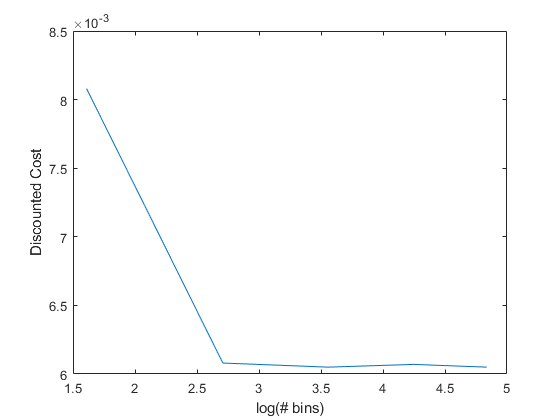
\includegraphics[height=5cm, width=8.75cm]{cost_5.png}
    \caption{Long-term discounted-cost of learned policies}
\end{figure}
\vspace{-1em}
\begin{figure}[H]
    \centering
    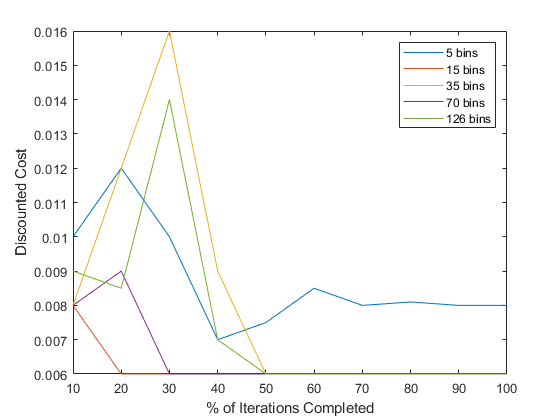
\includegraphics[height=5cm, width=8.75cm]{convergence_5.png}
    \caption{Convergece of learned policies}
\end{figure}

Note that the quantization gains are not significant after \( n=2 \) (which corresponds to 15 bins), which indicates that this is a sufficient quantization level for a near-optimal policy.
\newpage
Similarly, for 2-cell quantizers on \( \mathbb{X} = \{1,\ldots,16\} \),
\vspace{-1em}
\begin{figure}[H]
    \centering
    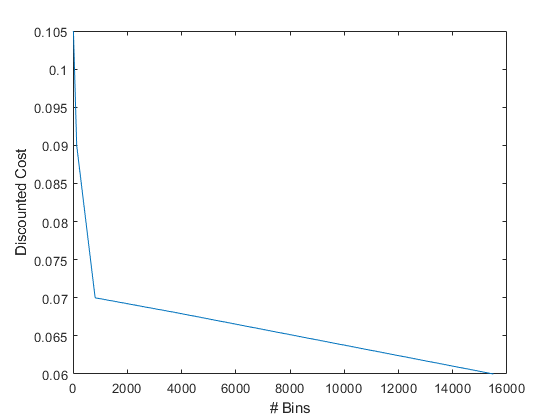
\includegraphics[height=5cm, width=8.75cm]{cost_16.png}
    \caption{Long-term discounted-cost of learned policies}
\end{figure}
\vspace{-1em}
\begin{figure}[H]
    \centering
    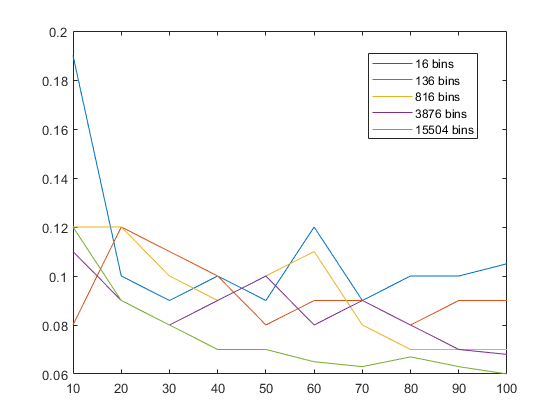
\includegraphics[height=5cm, width=8.75cm]{convergence_16.png}
    \caption{Convergece of learned policies}
\end{figure}

In this example, additional quantization may be required to get closer to the optimal policy.

\subsection{Comparison to Lloyd-Max Quantizer}
In these simulations, we plot the distortion for different values of \( n \) and for different quantizer rates (i.e. different sizes of \(\mathcal{M}\)). We also plot the comparison with a Lloyd-Max quantizer (another common algorithm to find an optimal quantizer), and note that our algorithm results in a lower discounted-cost. We use the source alphabet \( \mathbb{X} = \{1,\ldots,13\} \), and the rate is calculated by \(\log_2(|\mathcal{M}|)\).
\vspace{-1em}
\begin{figure}[H]
    \centering
    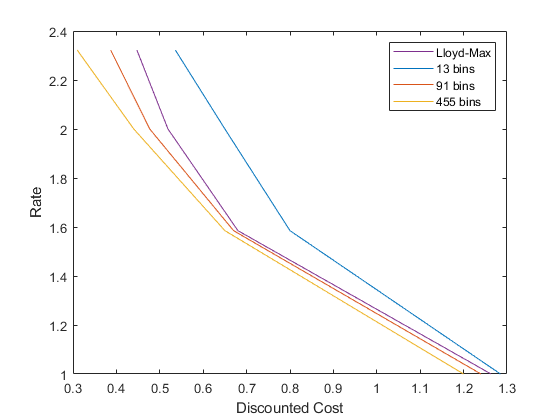
\includegraphics[height=5cm, width=8.75cm]{rate_distortion_lloydmax.png}
    \caption{Comparison with Lloyd-Max in Markov case}
\end{figure}

Note that for coarse quantizations, a Lloyd-Max quantizer may perform better, but as we increase the quantization, the Q-learning approach gives a lower distortion for a given rate.

Finally, we also note that our algorithm matches very closely with a Lloyd-Max quantizer in the case where the source is i.i.d., as can be seen below. Note that in this case, the Q-learning algorithm only visits one state (the one given by quantizing the distribution of \(X_0\)), and hence raising \(n\) provides no performance gain. Here we use \( \mathbb{X} = \{1,\ldots,8\} \).
\vspace{-1em}
\begin{figure}[H]
    \centering
    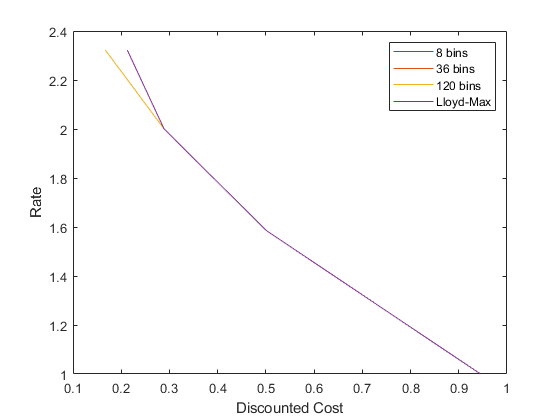
\includegraphics[height=5cm, width=8.75cm]{lloydmax_scalar.png}
    \caption{Comparison with Lloyd-Max in i.i.d. case}
\end{figure}

\noindent We now remark on the algorithm performance and feasibility:

\vspace{1em}
\noindent\emph{Remark 3.}\label{remark:3}
\begin{enumerate}
    \item As previously mentioned, the number of bins grows quickly with \(n\), and so running the algorithm with high \(n\) requires high amounts of memory in order to store a large Q-table. However, the number of actual visited \(\hat{\pi}_t\) tends to be much lower than the total number of bins, and so it may be possible to increase the efficiency of this algorithm by quantizing \( \pi_t \) in a non-uniform fashion (the results from~\cite{Kara} used for convergence of the algorithm allow a non-uniform quantization).
    \item As the number of bins grows, the time for the algorithm to converge becomes much higher, since it must visit more states. One must trade much longer algorithm runtime for potential performance increases. Also, since  we only have weak continuity of the transition kernel for \(\{\pi_t\}\), we do not have a bound on what quantization level we need to obtain a given performance (results from~\cite{Kara} provide these bounds under stronger notions of continuity). Therefore it is somewhat trial-and-error to find the appropriate quantization level for a given application.
    \item As mentioned in Section~\ref{section:optimal quantizers}, \(\{\pi_t\}\) updates in a Markovian fashion, and so we do not need to store the previous values of \(\pi_t\). Futhermore, from Section~\ref{section:unique-ergodicity} we have that the process \(\{\pi_t\}\) is stable (i.e. it ``forgets'' an incorrect prior) under the random exploration policy used in learning. Therefore we do not need to worry about errors accumulating over time, and in fact we can start the algorithm from any distribution \(\pi_0\) (the choice to initialize to the stationary distribution in \textbf{Algorithm 2} is just for convenience).
\end{enumerate}

\section{Future Work}
We would like to extend the algorithm to the case when \( \mathbb{X} \) is continuous. The primary obstable here would be that the number of possible quantizers is infinite, and so a method of quantizing the space of quantizers would need to be developed. We note however that quantizing the action space (in this context, the set of quantizers) is considered in the results from~\cite{Kara}, and also all of the predictor stability/unique invariance arguments in Section~\ref{section:unique-ergodicity} hold when \( \mathbb{X} \) is continuous. So with some minor alterations, the algorithm will still converge in the continuous case.

Finally, we wish to consider the case when the channel over which \(q_t\) is sent is noisy. While most of the results from Section~\ref{section:optimal quantizers} carry over in this case, additional considerations will have to be taken in other sections (e.g. in proving uniqueness of the invariant measure).

\appendix

\begin{theorem}\cite[Theorem 3.3]{NearOptimalityQuantized}\label{theorem:ACOE}
    Consider an MDP \((\mathsf{X}, \mathsf{U}, P, c)\), and suppose the following hold:
    \begin{enumerate}
        \item \(c\) is continuous, nonnegative, and bounded.
        \item \(\mathsf{U}\) is bounded.
        \item \(P(\cdot | x,u)\) is weakly continuous in \((x,u)\).
        \item \(\mathsf{X}\) is compact.
        \item The family of functions \(\{h_\beta : \beta \in (0,1)\}\), where
              \[h_\beta(x) := J^*_\beta(x) - J^*_\beta(x_0)\]
              for some fixed \(x_0 \in \mathsf{X}\), is uniformly bounded  and equicontinuous.
    \end{enumerate}
    Then there exist a constant \(g^* \ge 0\) and a measurable function \(f^* : \mathsf{X} \to \mathsf{U}\) such that the policy \(\gamma^* = \{f^*\}_{t\ge0}\) is optimal for the average-cost problem and \(g^*\) is the optimal value function, i.e.
    \[g^* = J^*(x) = J(x, \gamma^*)\]
    Furthermore, \(g^* = \lim_{n \to \infty}(1-\beta_n)J^*_{\beta_n}(x)\) for some sequence \(\{\beta_n\}_{n \ge 0}\) such that \(\beta_n \to 1\).
\end{theorem}

\subsection*{\textbf{Proof of Theorem~\ref{theorem:unique}}}
\begin{proof}
    Throughout, we use the notation \( \nu(f) := \int fd\nu \). Assume that \( m_1,m_2 \in \mathcal{P}(\mathbb{X} \times \mathcal{P}(\mathbb{X})) \) are two invariant measures for the joint process \( \{X_t,\pi_t^\nu \} \). Then their projections on \( \mathbb{X} \) are invariant for \( \{X_t\}_{t\ge0} \). Then, by unique invariance of \( \zeta(dx) \) we have
    \[ m_i(dx,d\nu) = P_{m_i}(d\nu | x)\zeta(dx) \]

    Then we show that \( m_1(F) = m_2(F) \) for each \( F \) on a set of measure-determining functions~\cite{Stettner}, namely those s.t. \( F(x,\nu) = \phi(x)H(\nu(\phi_1),\ldots,\nu(\phi_l)) \), where \( \phi \in C(\mathbb{X}), \phi_1,\ldots,\phi_l \in C(\mathbb{X}), H \) is bounded and Lipschitz continuous with constant \( L_H \), and \( l \in \mathbb{N} \).

    Let \( S \) be the transition operator associated with the process \( \{X_t,\pi_t \} \). Then by invariance we have for \( i=1,2 \):
    \[ m_i(F) = \smashoperator[l]{\int\limits_{\mathbb{X} \times \mathcal{P}(\mathbb{X})}} \frac{1}{n}\sum_{j=0}^{n-1}S^j F(x,\nu)P_{m_i}(d\nu | x)\zeta(dx) \]

    And thus,
    \begin{align*}
         & |m_1(F) - m_2(F)|                                                                                                                                                                                                                     \\
         & \le \int\limits_{\mathbb{X} \times \mathcal{P}(\mathbb{X}) \times \mathcal{P}(\mathbb{X})} \frac{1}{n}\sum_{j=0}^{n-1} |S^j F(x,\nu_1) - S^j F(x,\nu_2)|                                                                              \\ & \hspace{11em}\cdot P_{m_1}(x,\nu_1)P_{m_2}(x,v_2)\zeta(dx) \\
         & \le L_H ||\phi|| \quad\quad \smashoperator[l]{\int\limits_{\mathbb{X} \times \mathcal{P}(\mathbb{X}) \times \mathcal{P}(\mathbb{X})}} \frac{1}{n}\sum_{j=0}^{n-1}E^\mu[\sum_{i=1}^{l}|\pi_j^{\nu_1}(\phi_i) - \pi_j^{\nu_2}(\phi_i)|] \\ &\hspace{11em}\cdot P_{m_1}(x,\nu_1)P_{m_2}(x,v_2)\zeta(dx)
    \end{align*}
    Since the predictors are stable in the sense of Definition~\ref{definition:weak_stable}, and by the dominated convergence theorem, the last line converges to zero as \( n \to \infty \).
\end{proof}

Note that the above result concerns the joint process \( \{X_t,\pi_t \}_{t\ge0} \). The following theorem from~\cite{Stettner} extends this to \( \{\pi_t \}_{t\ge0} \).

\begin{theorem}\label{theorem:3.2}\cite[Theorem 3]{Stettner}
    If the joint process \( \{X_t,\pi_t \}_{t\ge0} \) is Feller and admits at most one invariant measure, then \( \{\pi_t\}_{t\ge0} \) admits at most one invariant measure.
\end{theorem}

Note that the above Feller assumption is trivially satisfied in the case where \( \mathbb{X} \) is finite, since \( \{\pi_t\}_{t\ge0} \) is Feller by Lemma~\ref{lemma:weak}.

\printbibliography
\end{document} %chktex 17